	\section{Цель работы}
		Требуется написать программу на языке FPTL, которая сжимает входную строку по алгоритму Хаффмана. 
	\section{Описание алгоритма}
		\lstinputlisting[caption={Программа на языке FPTL}]{listings/Haffman.txt}
	\section{Результаты}
		Информация о системе:
		\begin{itemize}
			\item Процессор: Intel® Core(TM) i7-4700HQ 2.4 GHz, 4 ядра;
			\item ОЗУ: 16,00 ГБ;
			\item Тип системы: 64 – разрядная;
		\end{itemize}

		\begin{figure}[h]
			\centering
			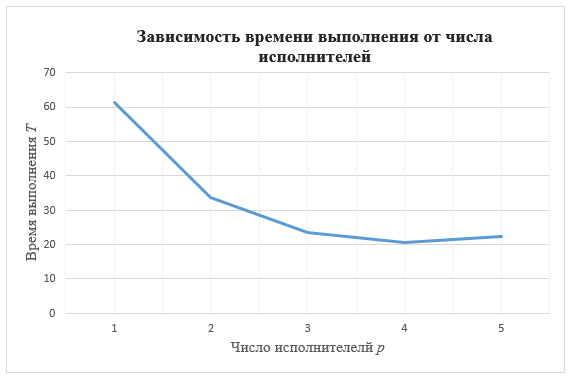
\includegraphics[width=1\linewidth]{images/time}
			\label{fig:time}
		\end{figure}
		\begin{figure}[h]
			\centering
			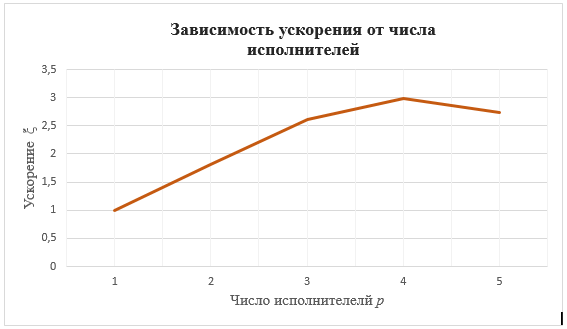
\includegraphics[width=1\linewidth]{images/acceleration}
			\label{fig:acceleration}
		\end{figure}
